\documentclass{article}

\usepackage{amsmath}
\usepackage[dvips]{graphicx}
\usepackage{verbatim}

\title{Stat 4201 HOMEWORK 1}
\author{Mengqi Zong $<mz2326@columbia.edu>$}


\begin{document}

\maketitle

\section{Question}
Consider the Salary Data (Display 1.3) in Ramsey \& Schafer, Chapter 1.
\begin{enumerate}
\item Determine whether there are outliers in the combined data, using
boxplots.
\item Perform separate EDA, and compute appropriate measures of
dispersion for the data in each group (i.e., Males and Females).
\item For each of the estimates computed in 2 above, determine the bias
and variance using each of the following methods:
\begin{itemize}
\item Jackknife
\item Bootstrap
\end{itemize}
\end{enumerate}

\section{Answers}

\subsection{Question 1}
The boxplot is show in Fig~\ref{fig:box_mix}. It shows that there is one
outlier in the combined data, it is "8100 MALE".

\begin{figure}[ht!]
  \centering
  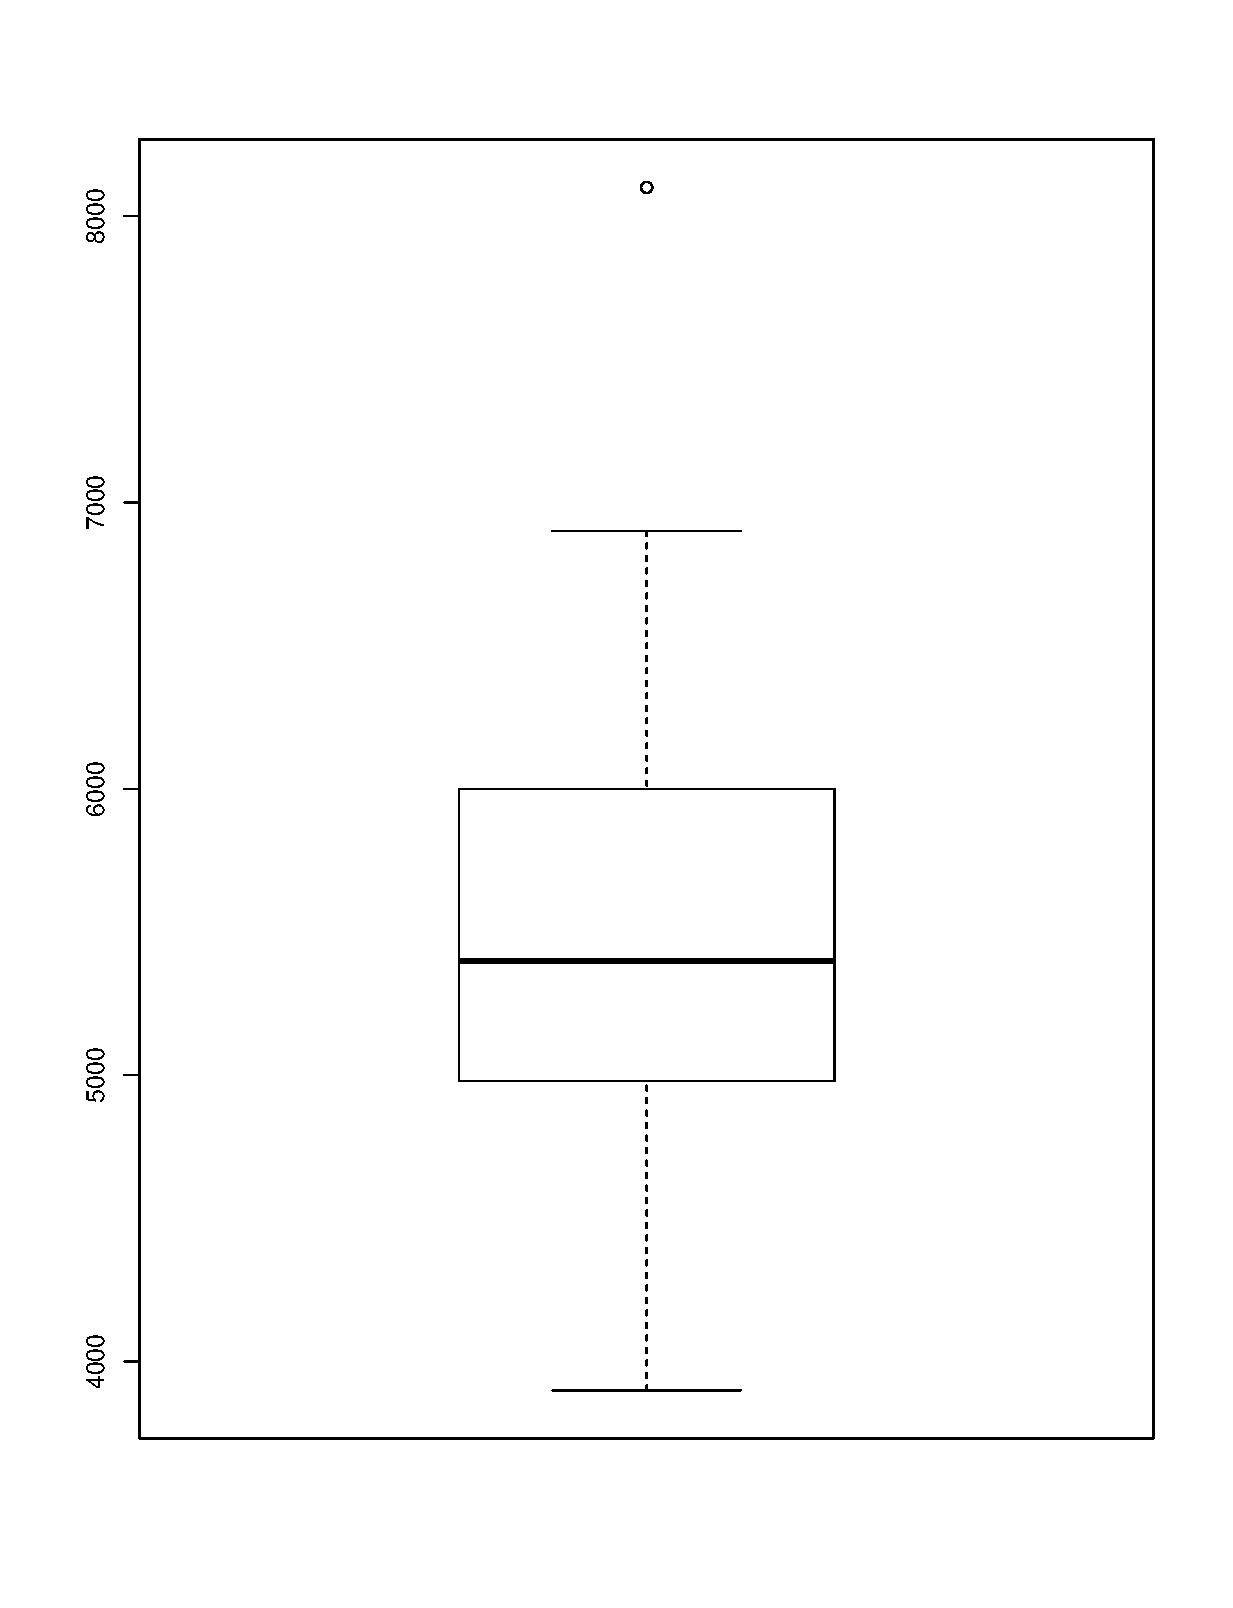
\includegraphics[width=0.7\textwidth]{boxplot_mix}
  \caption{Boxplot for the combined data \label{fig:box_mix}}
\end{figure}

\subsection{Question 2}

\subsubsection{EDA}
I use histograms, stem-and-leaf diagrams, and box plots. The histogram
for males is shown in Fig~\ref{fig:histm}, and the histogram for
females is shown in Fig-\ref{fig:hisf}. The box plot for males is
shown in Fig-\ref{fig:boxm}, and the box plot for females is shown in
Fig-\ref{fig:boxf}. As to the stem-and-leaf diagrams, the two diagrams
are listed below.\\

The stem-and-leaf diagram for males is:
\begin{verbatim}

  The decimal point is 3 digit(s) to the right of the |

  4 | 6
  5 | 011244444
  5 | 7
  6 | 00000000000003
  6 | 666899
  7 | 
  7 | 
  8 | 1

\end{verbatim}

The stem-and-leaf diagram for females is:
\begin{verbatim}

  The decimal point is 3 digit(s) to the right of the |

  4 | 6
  5 | 011244444
  5 | 7
  6 | 00000000000003
  6 | 666899
  7 | 
  7 | 
  8 | 1

\end{verbatim}

\begin{figure}[ht!]
  \centering
  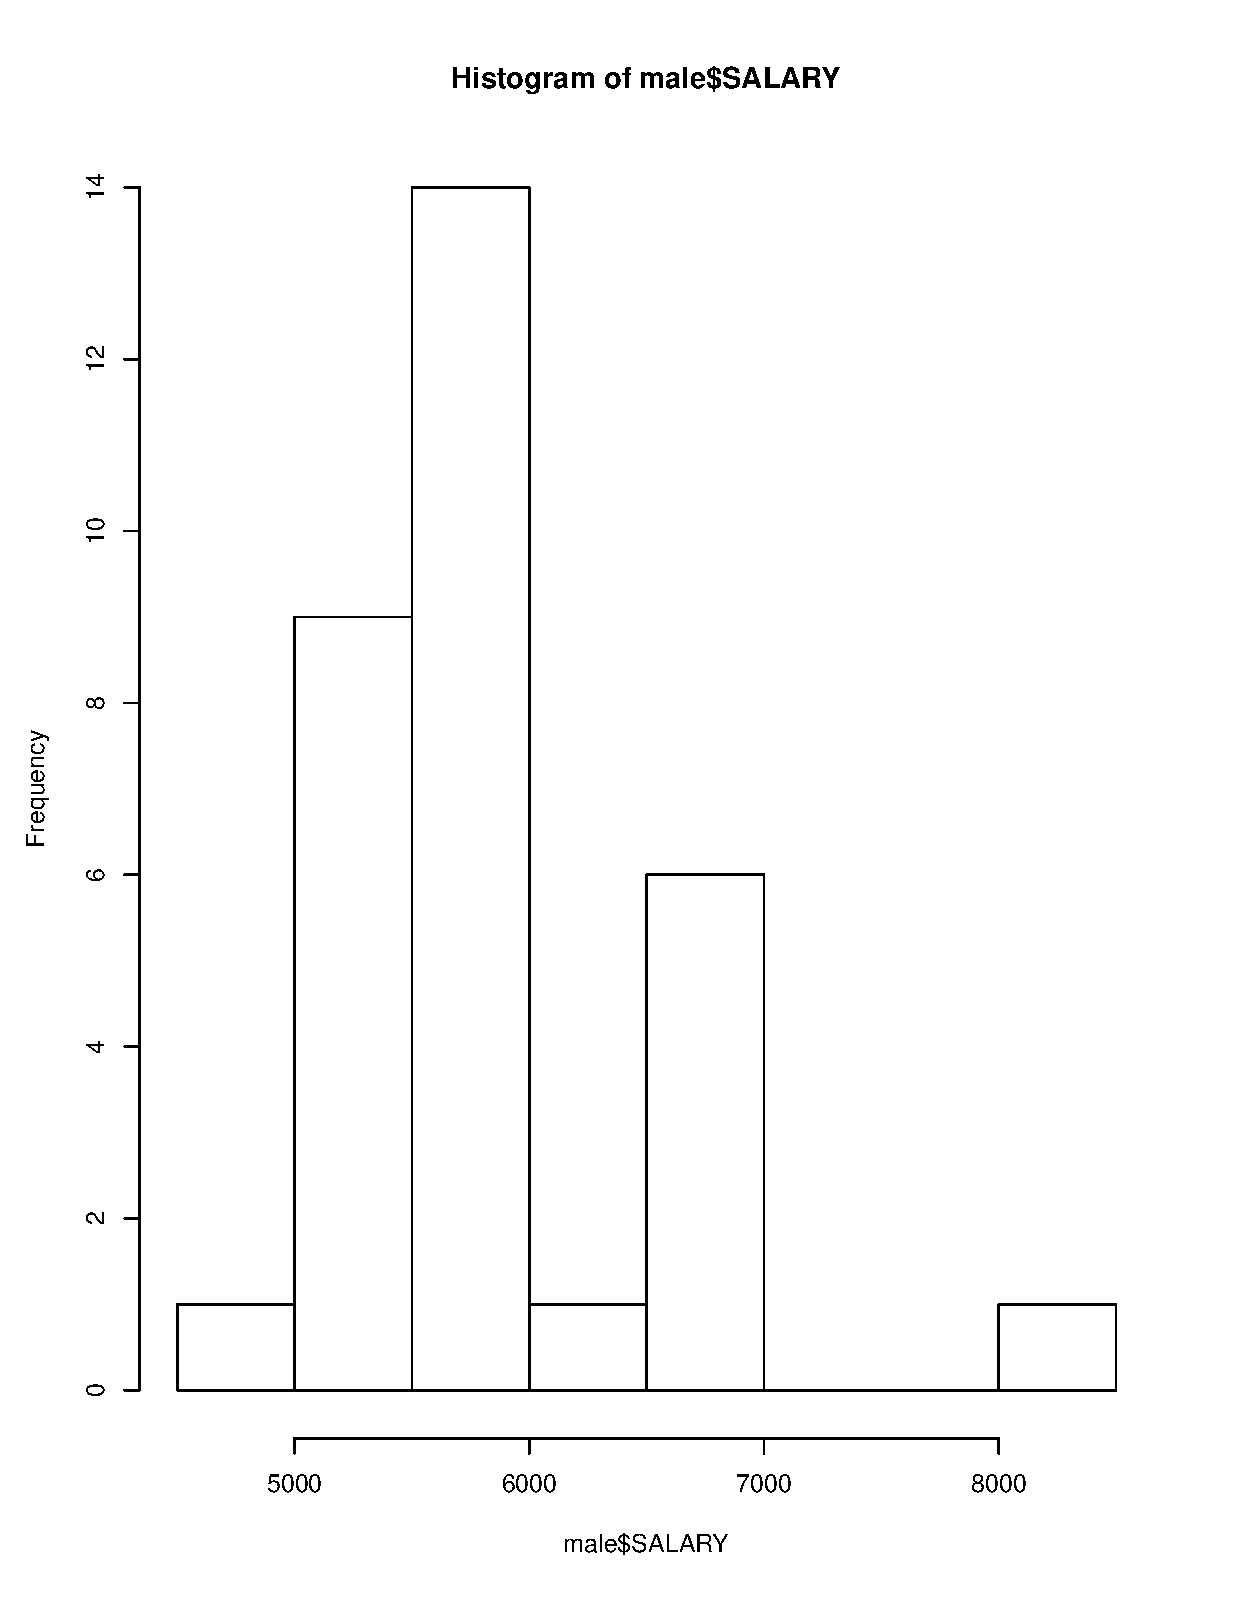
\includegraphics[width=0.7\textwidth]{hist_male}
  \caption{Histogram for male salaries \label{fig:histm}}
\end{figure}


\begin{figure}[ht!]
  \centering
  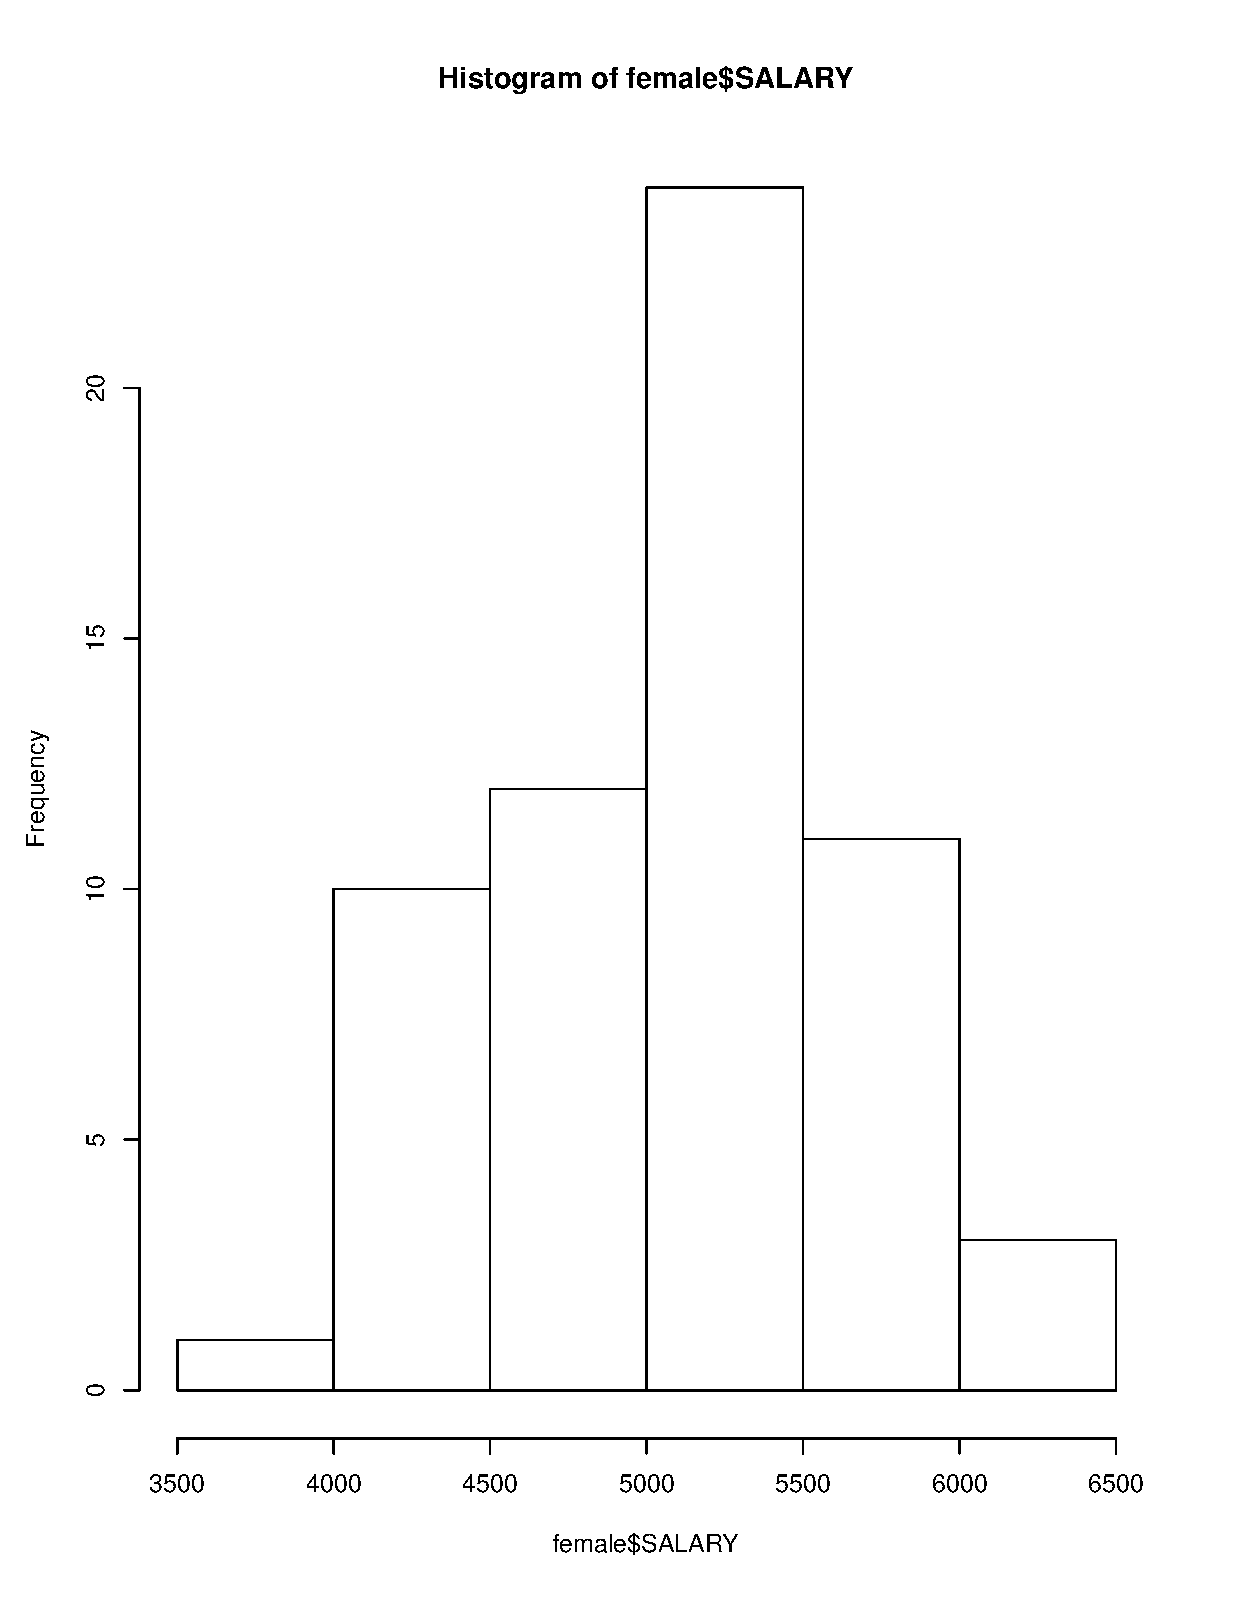
\includegraphics[width=0.7\textwidth]{hist_female}
  \caption{Histogram for female salaries \label{fig:histf}}
\end{figure}


\begin{figure}[ht!]
  \centering
  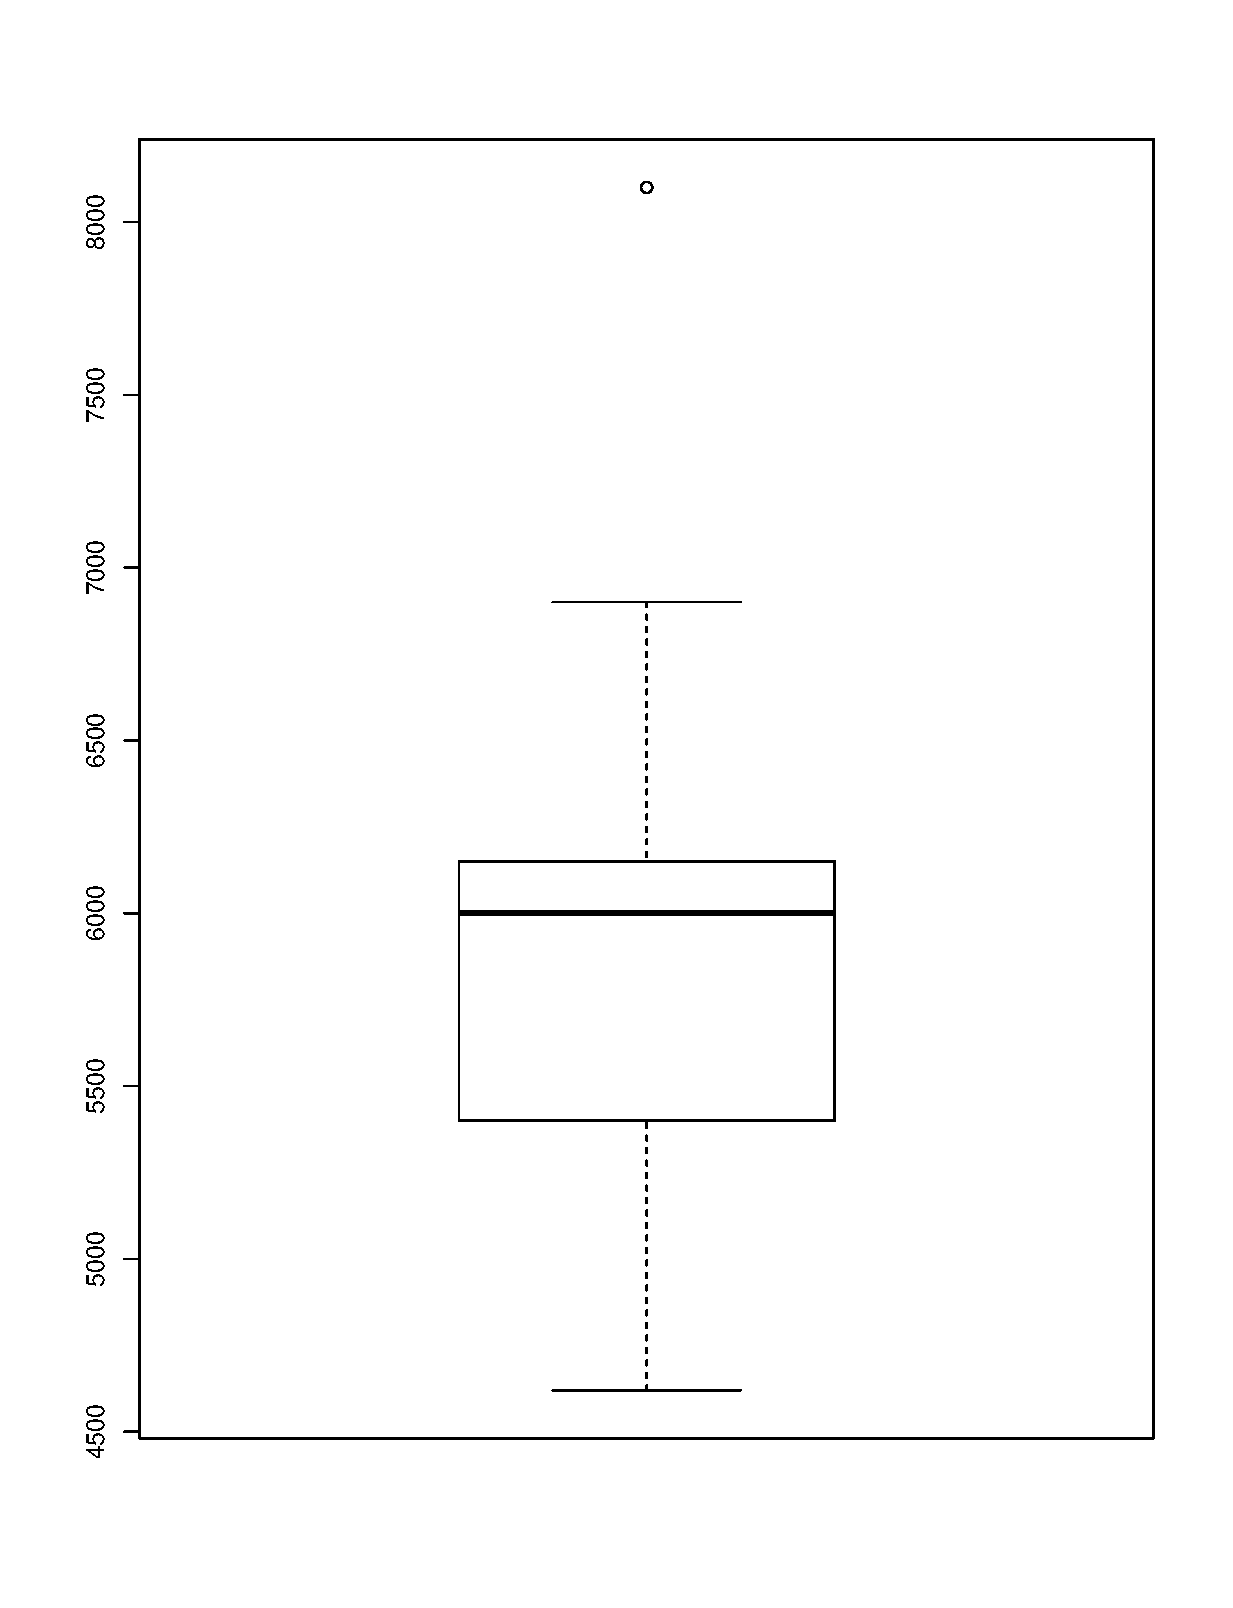
\includegraphics[width=0.7\textwidth]{boxplot_male}
  \caption{Boxplot for male salaries\label{fig:boxm}}
\end{figure}

\begin{figure}[ht!]
  \centering
  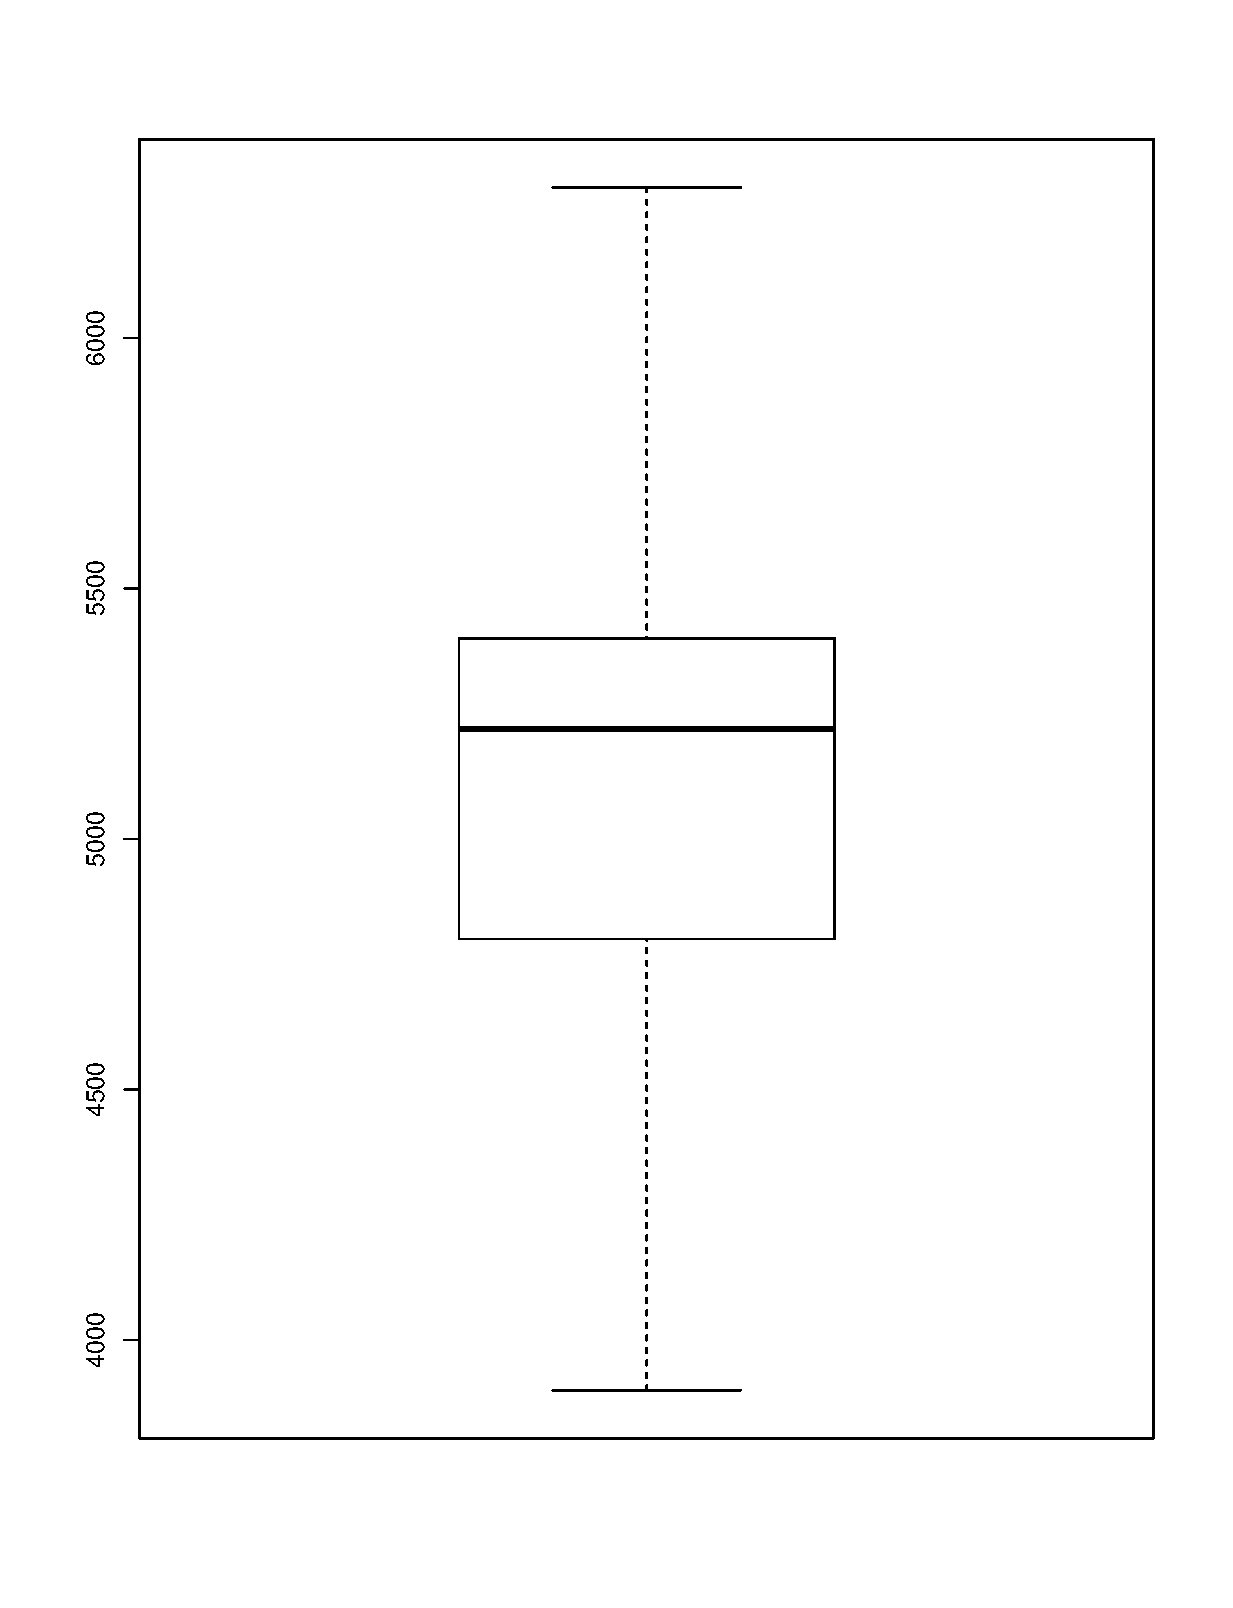
\includegraphics[width=0.7\textwidth]{boxplot_female}
  \caption{Boxplot for male salaries\label{fig:boxf}}
\end{figure}

\subsubsection{Measures of Dispersions}
I use standard deviation and interquartile range to measure the
dispersions. The calculated data is show in Table~\ref{tab:md}.

\begin{table}[ht!]
  \begin{center}
    \begin{tabular}{|l|c|c|}
                                                                 \hline
               &  Standard Deviation &  Interquartile Range   \\ \hline
      Males    &  690.7333           &    675                 \\ \hline
      Females  &  539.8707           &    600                 \\ \hline
    \end{tabular}
  \end{center}
  \caption{Measures of Dispersions \label{tab:md}}
\end{table}

\subsection{Question 3}
The summary of the estimated bias, variance is shown in
Table~\ref{tab:bv}.

\begin{table}[ht!]
\begin{center}
\begin{tabular}{|l|l|r|r|r|r|}
                                                  \hline
Method     & Variable        &  SD (M)   & IQL (M)  & SD (F)    & IQL (F) \\ \hline
Jackknife  & Bias            & -11.28011 &   1162.5 & -1.946738 & 0 \\ 
           & Standard Error  &  124.8158 & 361.6369 &  45.84659 & 0 \\ \hline
Bootstrap  & Bias            & -13.58164 &    46.47 & -9.533073 & 77.76 \\
           & Standard Error  &  117.2164 &  302.896 &  46.26237 & 126.0459 \\ \hline
    \end{tabular}
  \end{center}
  \caption{Measures of Dispersions \label{tab:bv}}
\end{table}

\section{Appendix}
The code is listed below:

\verbatiminput{hmwk1.r}
 
\end{document}
